\documentclass[10pt,a4paper]{report}
\usepackage[utf8]{inputenc}
\usepackage{amsmath}
\usepackage{amsfonts}
\usepackage{amssymb}
\usepackage{amsthm}
\usepackage{hyperref}

\usepackage{multicol}
\usepackage{fancyhdr}
\usepackage[inline]{enumitem}
\usepackage{tikz}
\usepackage{tikz-cd}
\usetikzlibrary{calc}
\usetikzlibrary{shapes.geometric}
\usetikzlibrary{positioning}
\usepackage[margin=0.5in]{geometry}
\usepackage{xcolor}

\hypersetup{
    colorlinks=true,
    linkcolor=blue,
    filecolor=magenta,      
    urlcolor=cyan,
    pdftitle={Tensors},
    pdfpagemode=FullScreen,
    }

%\urlstyle{same}

\newcommand{\CLASSNAME}{Math 5050 -- Special Topics: Manifolds}
\newcommand{\STUDENTNAME}{Paul Carmody}
\newcommand{\ASSIGNMENT}{Notes }
\newcommand{\DUEDATE}{January -- May, 2025}
\newcommand{\SEMESTER}{Spring 2025}
\newcommand{\SCHEDULE}{MW 12:30 - 1:45}
\newcommand{\ROOM}{Remote}

\newcommand{\MMN}{M_{m\times n}}
\newcommand{\FF}{\mathcal{F}}

\pagestyle{fancy}
\fancyhf{}
\chead{ \fancyplain{}{\CLASSNAME} }
%\chead{ \fancyplain{}{\STUDENTNAME} }
\rhead{\thepage}
\newcommand{\LET}{\text{Let }}
%\newcommand{\IF}{\text{if }}
\newcommand{\AND}{\text{ and }}
\newcommand{\OR}{\text{ or }}
\newcommand{\FORSOME}{\text{ for some }}
\newcommand{\FORALL}{\text{ for all }}
\newcommand{\WHERE}{\text{ where }}
\newcommand{\WTS}{\text{ WTS }}
\newcommand{\WLOG}{\text{ WLOG }}
\newcommand{\BS}{\backslash}
\newcommand{\DEFINE}[1]{\textbf{\emph{#1}}}
\newcommand{\IF}{$(\Rightarrow)$}
\newcommand{\ONLYIF}{$(\Leftarrow)$}
\newcommand{\ITH}{\textsuperscript{th} }
\newcommand{\FST}{\textsuperscript{st} }
\newcommand{\SND}{\textsuperscript{nd} }
\newcommand{\TRD}{\textsuperscript{rd} }
\newcommand{\INV}{\textsuperscript{-1} }

\newcommand{\XXX}{\mathfrak{X}}
\newcommand{\MMM}{\mathfrak{M}}
%\newcommand{\????}{\textfrak{A}}
%\newcommand{\????}{\textgoth{A}}
%\newcommand{\????}{\textswab{A}}

\DeclareMathOperator{\DER}{Der}
\DeclareMathOperator{\SGN}{sgn}

%%%%%%%
% derivatives
%%%%%%%

\newcommand{\PART}[2]{\frac{\partial #1}{\partial #2}}
\newcommand{\SPART}[2]{\frac{\partial^2 #1}{\partial #2^2}}
\newcommand{\DERIV}[2]{\frac{d #1}{d #2}}
\newcommand{\LAPLACIAN}[1]{\frac{\partial^2 #1}{\partial x^2} + \frac{\partial^2 #1}{\partial y^2}}

%%%%%%%
% sum, product, union, intersections
%%%%%%%

\newcommand{\SUM}[2]{\underset{#1}{\overset{#2}{\sum}}}
\newcommand{\PROD}[2]{\underset{#1}{\overset{#2}{\prod}}}
\newcommand{\UNION}[2]{\underset{#1}{\overset{#2}{\bigcup}}}
\newcommand{\INTERSECT}[2]{\underset{#1}{\overset{#2}{\bigcap}}}
\newcommand{\FSUM}{\SUM{n=-\infty}{\infty}}
       

%%%%%%%
% supremum and infimum
%%%%%%%

\newcommand{\SUP}[1]{\underset{#1}\sup \,}
\newcommand{\INF}[1]{\underset{#1}\inf \,}
\newcommand{\MAX}[1]{\underset{#1}\max \,}
\newcommand{\MIN}[1]{\underset{#1}\min \,}

%%%%%%%
% infinite sums, limits
%%%%%%%

\newcommand{\SUMK}{\SUM{k=1}{\infty}}
\newcommand{\SUMN}{\SUM{n=1}{\infty}}
\newcommand{\SUMKZ}{\SUM{k=0}{\infty}}
\newcommand{\LIM}[1]{\underset{#1}\lim\,}
\newcommand{\IWOB}[1]{\LIM{#1 \to \infty}}
\newcommand{\LIMK}{\IWOB{k}}
\newcommand{\LIMN}{\IWOB{n}}
\newcommand{\LIMX}{\IWOB{x}}
\newcommand{\NIWOB}{\LIM{n \to \infty}}
\newcommand{\LIMSUPK}{\underset{k\to\infty}\limsup \,}
\newcommand{\LIMSUPN}{\underset{n\to\infty}\limsup \,}
\newcommand{\LIMINFK}{\underset{k\to\infty}\liminf \,}
\newcommand{\LIMINFN}{\underset{n\to\infty}\liminf \,}
\newcommand{\ROOTRULE}[1]{\LIMSUPK \BARS{#1}^{1/k}}

\newcommand{\CUPK}{\bigcup_{k=1}^{\infty}}
\newcommand{\CAPK}{\bigcap_{k=1}^{\infty}}
\newcommand{\CUPN}{\bigcup_{n=1}^{\infty}}
\newcommand{\CAPN}{\bigcap_{n=1}^{\infty}}

%%%%%%%
% number systems (real, rational, etc.)
%%%%%%%

\newcommand{\REALS}{\mathbb{R}}
\newcommand{\RATIONALS}{\mathbb{Q}}
\newcommand{\IRRATIONALS}{\REALS \backslash \RATIONALS}
\newcommand{\INTEGERS}{\mathbb{Z}}
\newcommand{\NUMBERS}{\mathbb{N}}
\newcommand{\COMPLEX}{\mathbb{C}}
\newcommand{\DISC}{\mathbb{D}}
\newcommand{\HPLANE}{\mathbb{H}}

\newcommand{\R}{\mathbb{R}}
\newcommand{\Q}{\mathbb{Q}}
\newcommand{\Z}{\mathbb{Z}}
\newcommand{\N}{\mathbb{N}}
\newcommand{\C}{\mathbb{C}}
\newcommand{\T}{\mathbb{T}}
\newcommand{\COUNTABLE}{\aleph_0}
\newcommand{\UNCOUNTABLE}{\aleph_1}


%%%%%%%
% Arithmetic/Algebraic operators
%%%%%%%


\DeclareMathOperator{\MOD}{mod}
%\newcommand{\MOD}[1]{\mod #1}
\newcommand{\BAR}[1]{\overline{#1}}
\newcommand{\LCM}{\text{ lcm}}
\newcommand{\ZMOD}[1]{\Z/#1\Z}
\DeclareMathOperator{\VAR}{Var}
%%%%%%%
% complex operators
%%%%%%%

\DeclareMathOperator{\RR}{Re}
%\newcommand{\RE}{\text{Re}}
\DeclareMathOperator{\IM}{Im}
%\newcommand{\IM}{\text{Im}}
\newcommand{\CONJ}[1]{\overline{#1}}
\DeclareMathOperator{\LOG}{Log}
%\newcommand{\LOG}{\text{ Log }}
\newcommand{\RES}[2]{\underset{#1}{\text{res}} #2}

%%%%%%%
% Group operators
%%%%%%%

\newcommand{\AUT}{\text{Aut}\,}
\newcommand{\KER}{\text{ker}\,}
\newcommand{\END}{\text{End}}
\newcommand{\HOM}{\text{Hom}}
\newcommand{\CYCLE}[1]{(\begin{array}{cccccccccc}
		#1
	\end{array})}
\newcommand{\SUBGROUP}{\underset{\text{group}}\subseteq}	
%\newcommand{\SUBGROUP}{\subseteq_g}
\newcommand{\SUBRING}{\underset{\text{ring}}\subseteq}
\newcommand{\SUBMOD}{\underset{\text{mod}}\subseteq}
\newcommand{\SUBFIELD}{\underset{\text{field}}\subseteq}
\newcommand{\ISO}{\underset{\text{iso}}\longrightarrow}
\newcommand{\HOMO}{\underset{\text{homo}}\longrightarrow}

%%%%%%%
% grouping (parenthesis, absolute value, square, multi-level brackets).
%%%%%%%

\newcommand{\PAREN}[1]{\left (\, #1 \,\right )}
\newcommand{\BRACKET}[1]{\left \{\, #1 \,\right \}}
\newcommand{\SQBRACKET}[1]{\left [\, #1 \,\right ]}
\newcommand{\ABRACKET}[1]{\left \langle\, #1 \,\right \rangle}
\newcommand{\BARS}[1]{\left |\, #1 \,\right |}
\newcommand{\DBARS}[1]{\left \| \, #1 \,\right \|}
\newcommand{\LBRACKET}[1]{\left \{ #1 \right .} 
\newcommand{\RBRACKET}[1]{\left . #1 \right \]}
\newcommand{\RBAR}[1]{\left . #1 \, \right |}
\newcommand{\LBAR}[1]{\left | \, #1 \right .}
\newcommand{\BLBRACKET}[2]{\BRACKET{\RBAR{#1}#2}}
\newcommand{\GEN}[1]{\ABRACKET{#1}}
\newcommand{\BINDEF}[2]{\LBRACKET{\begin{array}{ll}
     #1\\
     #2
\end{array}}}

%%%%%%%
% Fourier Analysis
%%%%%%%

\newcommand{\ONEOTWOPI}{\frac{1}{2\pi}}
\newcommand{\FHAT}{\hat{f}(n)}
\newcommand{\FINT}{\int_{-\pi}^\pi}
\newcommand{\FINTWO}{\int_{0}^{2\pi}}
\newcommand{\FSUMN}[1]{\SUM{n=-#1}{#1}}
%\newcommand{\FSUM}{\SUMN{\infty}}
\newcommand{\EIN}[1]{e^{in#1}}
\newcommand{\NEIN}[1]{e^{-in#1}}
\newcommand{\INTALL}{\int_{-\infty}^{\infty}}
\newcommand{\FTINT}[1]{\INTALL #1 e^{2\pi inx\xi} dx}
\newcommand{\GAUSS}{e^{-\pi x^2}}

%%%%%%%
% formatting 
%%%%%%%

\newcommand{\LEFTBOLD}[1]{\noindent\textbf{#1}}
\newcommand{\SEQ}[1]{\{#1\,\}}
\newcommand{\WIP}{\footnote{work in progress}}
\newcommand{\QED}{\hfill\square}
\newcommand{\ts}{\textsuperscript}
\newcommand{\HLINE}{\noindent\rule{7in}{1pt}\\}

%%%%%%%
% Mathematical note taking (definitions, theorems, etc.)
%%%%%%%

\newcommand{\REM}{\noindent\textbf{\\Remark: }}
\newcommand{\DEF}{\noindent\textbf{\\Definition: }}
\newcommand{\THE}{\noindent\textbf{\\Theorem: }}
\newcommand{\COR}{\noindent\textbf{\\Corollary: }}
\newcommand{\LEM}{\noindent\textbf{\\Lemma: }}
\newcommand{\PROP}{\noindent\textbf{\\Proposition: }}
\newcommand{\PROOF}{\noindent\textbf{\\Proof: }}
\newcommand{\EXP}{\noindent\textbf{\\Example: }}
\newcommand{\TRICKS}{\noindent\textbf{\\Tricks: }}


%%%%%%%
% text highlighting
%%%%%%%

\newcommand{\B}[1]{\textbf{#1}}
\newcommand{\CAL}[1]{\mathcal{#1}}
\newcommand{\UL}[1]{\underline{#1}}

%%%%%%
% Linear Algebra
%%%%%%

\newcommand{\COLVECTOR}[1]{\PAREN{\begin{array}{c}
#1
\end{array} }}
\newcommand{\TWOXTWO}[4]{\PAREN{ \begin{array}{c c} #1&#2 \\ #3 & #4 \end{array} }}
\newcommand{\DTWOXTWO}[4]{\BARS{ \begin{array}{c c} #1&#2 \\ #3 & #4 \end{array} }}
\newcommand{\THREEXTHREE}[9]{\PAREN{ \begin{array}{c c c} #1&#2&#3 \\ #4 & #5 & #6 \\ #7 & #8 & #9 \end{array} }}
\newcommand{\DTHREEXTHREE}[9]{\BARS{ \begin{array}{c c c} #1&#2&#3 \\ #4 & #5 & #6 \\ #7 & #8 & #9 \end{array} }}
\newcommand{\NXN}{\PAREN{ \begin{array}{c c c c} 
			a_{11} & a_{12} & \cdots & a_{1n} \\
			a_{21} & a_{22} & \cdots & a_{2n} \\
			\vdots & \vdots & \ddots & a_{1n} \\
			a_{n1} & a_{n2} & \cdots & a_{nn} \\
		\end{array} }}
\newcommand{\SLR}{SL_2(\R)}
\newcommand{\GLR}{GL_2(\R)}
\DeclareMathOperator{\TR}{tr}
\DeclareMathOperator{\BIL}{Bil}
\DeclareMathOperator{\SPAN}{span}

%%%%%%%
%  White space
%%%%%%%

\newcommand{\BOXIT}[1]{\noindent\fbox{\parbox{\textwidth}{#1}}}


\newtheorem{theorem}{Theorem}[section]
\newtheorem{corollary}{Corollary}[theorem]
\newtheorem{lemma}[theorem]{Lemma}

\theoremstyle{definition}
\newtheorem{definition}[theorem]{Definition}
\newtheorem{prop}[theorem]{Proposition}

\theoremstyle{remark}
\newtheorem{remark}[theorem]{Remark}
\newtheorem{example}[theorem]{Example}
%\newtheorem*{proof}[theorem]{Proof}



\newcommand{\RED}[1]{\textcolor{red}{#1}}
\newcommand{\BLUE}[1]{\textcolor{blue}{#1}}

\begin{document}

\begin{center}
	\Large{\CLASSNAME -- \SEMESTER} \\
	\large{ w/Professor Berchenko-Kogan}
\end{center}
\begin{center}
	\STUDENTNAME \\
	\ASSIGNMENT -- \DUEDATE\\
\end{center} 

\noindent \textbf{Definitions}

\begin{enumerate}
	\item \DEFINE{Diffeomorphism}: If $f \in C^\infty$ and $f^{-1} \in C^\infty$ then $f$ is said to be a \DEFINE{diffeomorphism}.  Similarly, if there exists a mapping between two sets that is a diffeomorphism, the sets are said to be \DEFINE{diffeomorphic} to each other.
	\item \DEFINE{Tangent Space} at a point $p$.  The set of all vectors rooted at $p$, written as $T_p(\R^n)$.  
	\item \DEFINE{Derivations}: any operation that supports the Liebniz Rule ($D(fg) = (Df)g+fDg$).
	\item \DEFINE{Derivation Space}. $\mathcal{D}_p(\R^n)$ is the set of all derivations at $p$.  This constitutes a vector space.  There exists an isomorphism $\phi: T_p(\R^n) \to \mathcal{D}(\R^n)$ defined as
	\begin{align*}
		\phi: T_p(\R^n) &\to \mathcal{D}_p(\R^n)\\
		v &\mapsto D_v=\sum v^i \RBAR{\PART{}{x^i}}_p.
	\end{align*}
	\item \DEFINE{Germ}: equivalence class of functions whose derivatives around a point are the same.
	\item Vector Field vs Vector Space.  
	\begin{itemize}
		\item \DEFINE{A Vector Field} a function that assigns a vector to every point in the subset $U$. 
		\begin{align*}
			f: (U\subset \R^m) &\to T_p( \R^n) \\
				X &\mapsto X_p=\sum \RBAR{a^i(p) \PART{}{x^i} }_p.
		\end{align*}consider $a^i$ as coefficent functions.  We say that $X$ is $C^\infty$ on $U$ if $a^i\in C^\infty, \, \forall i=1,\dots,n$.
		\item \DEFINE{A Vector Space} is any abstraciton that is closed under addition and scalar multiplication.
	\end{itemize}
	\item \DEFINE{Dual Basis and Dual Space}.  The \DEFINE{Dual Basis} is a set of functions $\alpha^i: V \to \R$ 
	\begin{align*}
		\alpha^i &: V \to \R \\
			\alpha^i(e_j) &= \delta_j^i
	\end{align*}the \DEFINE{Dual Space $V^\vee$} is the space of functions spanned by the Dual Basis. Elements of the Dual Space are called \DEFINE{Functionals (Analysis)/1-Covectors (Differential Geometry)}.  
	\item \DEFINE{Multi-Linear Functions and Vector Space of k-tensors $L_k(V)$} Let $V$ be a vector space and $V^k$ be $k$-tuples of vectors in $V$. A \DEFINE{$K$-linear map or $k$-tensor} $f: V^k \to \R$ such that each $i$\textsuperscript{th} component is linear.  The vector space of all $k$-tensors on $V$ is denoted $L_k(V)$.
	
	\textbf{Permuting Mult-linear Functions}.  Given any permutation $\sigma \in S_k$
	\begin{align*}
		f(v_1, \dots, v_k) &= f(v_{\sigma(1)}, \dots, v_{\sigma(k)})
	\end{align*}e.g., $f(x,y,z) = xyz \to f(z,x,y) = zxy$.  FYI: if $x,y,z$ are from non-commutative rings (i.e., matrices) then we must be aware of the $\SGN(\sigma)$.
	
	\item Left \DEFINE{$R$-Module}: An Abelian group $R$ with a scalar multiplication map:
	\begin{align*}
		\mu : R \times A \to A
	\end{align*}usually written as $\mu(r,a)$, such that $r,s \in \R$ and $a,b \in A$	 a
	\begin{enumerate}[label=(\roman*)]
		\item (associative) $(rs)a = r(sa)$.
		\item (identity) $1a = a$ (1 is a multiplicative identity).
		\item (distributivity) $(r+s)a = ra+sa$ and $r(a+b) = ra+rb$.	
	\end{enumerate}	 If $R$ is a field then $R$-module is precisely a vector space over $R$.
	
	A \DEFINE{$K$-Algebra over a field $K$} is also a ring $A$ that is also a vector space over $K$ such that the ring multiplication satisfies homogeniety (scalar distributes over vector multipliation to only one of the operators).
	
	A \DEFINE{graded Algebra} is an algebra $A$ over a field $K$ if it can be writte as the direct sum $$ A = \bigoplus_{i=0}^\infty A^i$$ of vector spaces over $K$ such that the mupltiplication map sends $A^k \times A^l \to A^{k+l}$
	
	\item The set of all $C^\infty$-vector fields on $U$, denoted by $\XXX(U)$, is not only a vector space over $\R$, but also a \textit{module} over the $C^\infty(U)$ ring. \begin{align*}
		\XXX(U) &= \BRACKET{ X : V \to V \;|\; X \in C^\infty(U)} \text{ where } V = (\R \OR \C)^n
	\end{align*}
	\item \DEFINE{Derivation: } A \DEFINE{derivation} on an algebra $A$ is a $K$-multilinear function $D:A \to A$ such that 
	\begin{align*}
		D(ab) &= (Da)b+aDb, \, \forall a,b \in A
	\end{align*}known as the \DEFINE{Liebniz Rule}.
	
	The set of all derivations on $A$ forms a vector space, $\DER(C^\infty(U))$.  Thus a $C^\infty(U)$ vector field gives rise to a derivation of the algebra $C^\infty(U)$.  Thus the mapping
	\begin{align*}
		\varphi : \XXX(U) &\to \DER(C^\infty(U)) \\
		X &\mapsto (f\mapsto Xf)
	\end{align*}this map is an isomorphism of vector spaces.
	\item \textbf{Exterior Algebras $\Lambda(V)$.} The exterior algebra $\Lambda(V)$ is obtained by imposing an \textbf{anti-commutative} relation: 
	\begin{align*}
		v\otimes w + w\otimes v = 0,\, \forall v,w \in V
	\end{align*}this means that the quotient algebra is:
	\begin{align*}
		\Lambda(V) &= T(V)/\ABRACKET{v\otimes w + w\otimes v}.
	\end{align*}Where $T(V)$ is the \textbf{tensor algebra}
	\begin{align*}
		T(V) &= \bigoplus_{n=1}^\infty V^{\otimes n}
	\end{align*}
	\item \textbf{Symmetric Algebras $S(V)$.} The symmetric algebra $S(V)$ is obtained by imposing an \textbf{commutative} relation: 
	\begin{align*}
		v\otimes w - w\otimes v = 0,\, \forall v,w \in V
	\end{align*}this means that the quotient algebra is:
	\begin{align*}
		S(V) &= T(V)/\ABRACKET{v\otimes w - w\otimes v}.
	\end{align*}
	\item \DEFINE{Tensor Product} The tensor product between two 1-covectors, $f,g: V \to \R$ is the 2-covector $f\otimes g$.
	\begin{align*}
		(f \otimes g)(u,v) &= f(u)g(v)
	\end{align*}.  In general, the tensor product of a $k$-covector $p:V^k \to \R$ with a $l$-covector $q:v^l \to \R$ is the $(k+l)$-covector $p\otimes q: V^{k+l}\to \R$.
	\begin{align*}
		(p\otimes q)(u,v) = p(u)q(v),\,\forall u\in V^k,\, v\in V^l
	\end{align*}
	\item \DEFINE{Tensor Product(?)} is an operator on $v \in V$ and $u \in U$ where 
	\begin{align*}
		v \otimes u &: V \times U \to V \oplus U \\
		(v \otimes u)_{i\cdot j} &= v_i \cdot u_j,\, \forall i=1,\dots,\dim(V),\, j=1,\dots,\dim(U)
	\end{align*}
	
	Given two vector spaces $V, W$ with bases $v_1, \dots, v_n$ and $w_1, \dots, w_m$ then the Tensor Product space $V \otimes W$ has a basis referred to as $v_i \otimes w_j$ such that given any vector $\alpha = \sum \alpha_i v_i \in V$ and $\beta = \sum \beta_j w_j \in W$ the vector $\alpha \otimes \beta$ will have $n\times m$ components and each $(\alpha \otimes \beta)_{i\times j} = \alpha_i \times \beta_j$.\\
	\\
	$\alpha_i, \beta_j$ are all scalars.  The real issue is the behavior of unit basis vectors $v_i, w_j$ and how they are effected by the operator and the basis vectors $v_i \otimes w_j$.  Thus, scalar multiplication works on either (but not both) operands and distribution over addition works over both the left and the right.
	\item \DEFINE{Wedge Product }
	\begin{description}
		\item \textbf{Between two covectors} Let $f,g \in L_1(V)$ then for all $u,v \in V$
		\begin{align*}
			(f\wedge g)(u,v) &= (f\otimes g)(u,v) - (g \otimes f)(u,v) = f(u)g(v) - f(v)g(u)
		\end{align*}
	\item \textbf{Between mulitple 1-covectors. }
	\begin{align*}
		(\alpha^1\otimes\cdots\otimes\alpha^k)(v_1,\dots,v_k) &= \det[\alpha^1(v_j)] \\
		&= \sum_{\sigma \in S_k} (\SGN \sigma)\alpha_1(v_{\sigma(1)})\cdots\alpha_k(v_{\sigma(k)})
	\end{align*}
	\item \textbf{Between $k$-covector and $l$-covector}.  Let $f \in A_k(V)$, $g \in A_l(V)$ then
	\begin{align*}
		f \wedge g &= \frac{1}{k!l!}A(f \otimes g) \in A_{k+l}(V)
	\end{align*} or explicitly
	\begin{align*}
		(f\wedge g)(v_1, \dots, v_{k+l}) &= \frac{1}{k!l!}\sum_{\sigma \in S_{k+l}} f\PAREN{v_{\sigma{1}},\dots, v_{\sigma_{k}}}\, g\PAREN{v_{\sigma_{k+1}},\dots,v_{\sigma{k+l}}}
	\end{align*}
	\item \textbf{Anticommutative.}  Let $f \in A_k(V)$, $g \in A_l(V)$ then
	\begin{align*}
		(f \wedge g) = (-1)^{kl} g \wedge f
	\end{align*}

	\end{description}
	\item \textbf{Differential k-Forms} 
	
	\textbf{1-forms, covectors } 
	\begin{align*}
		(dx^i)\PAREN{\RBAR{\PART{}{x^j}}_p} &= \RBAR{\PART{}{x^j}}_p x^i = \delta_j^i\\
		(df)_p(X_p) &= X_p f = \sum \RBAR{a^i(p) \PART{f}{x^i} }_p =\sum \PART{}{x^i} dx^i
	\end{align*}
	\item \textbf{$\Omega^k(U)$, Vector space of $C^\infty\, k$-forms on U}.
	\begin{description}
		\item $\Omega^0 = A_0(T_p(\R^n)) = C^\infty(U)$, e.g., $f\in \Omega^0$ then $f: V \to \R$ is a functional/covector/1-tensor.
		\item Elements of 1-form $\Omega^1 = A_1(T_p(\R^n))$.  For example, when $n=3$
		\begin{align*}
			fdx+gdy+hdz,\text{ where }f,g,h \in C^\infty(\R^3)
		\end{align*}
		\item Elements of 2-form $\Omega^2 = A_2(T_p(\R^n))$.  For example, when $n=3$\footnote{NOTE the cyclic order of the indices $x,y,z$.  Switching any one of these will flip the sign.}
		\begin{align*}
			fdy\wedge dz+gdx\wedge dz+hdx\wedge dy,\text{ where }f,g,h \in C^\infty(\R^3)
		\end{align*}
		\item if $n=4$, that is coordinates for $u,v,w,x$. Each form is derived from these bases 
		
		0-form $\Omega^0(\R^4)\in \R$ 
		
		1-forms $\Omega^1(\R^4)$ summing $du, dv, dw, dx$, 
		
		2-forms $\Omega^2(\R^4)$ summing  $du\wedge dv,\, du \wedge dw,\, du \wedge dx,\, dv \wedge dw,\, dv \wedge dx,\, dw \wedge dx$, 
		
		3-forms $\Omega^3(\R^4)$ summing $du\wedge dv \wedge dw\;|\; du \wedge dw \wedge dx\;| \; du\wedge dv \wedge dx\;|\; dv \wedge dw \wedge dx$
		
		4-form $\Omega^4(\R^4)$ $du\wedge dv\wedge dw\wedge dx$.
		\item Also, \textbf{$U\subseteq\R^n$ then $k<n$}.  $k$-forms for $k>n$ are zero.  Further $|\Omega^k(\R^n)|=\binom{k}{n}$ and $\BARS{\bigcup_k \Omega^k(\R^n)}=2^n$	 and think of $\Omega^*(U)= \bigcup_k \Omega^k(\R^n)$
		\item \textbf{Direct Sum. } $\Omega^*(U) = \bigoplus_k \Omega^k(U)$ is an anti-commutative graded algebra over $\R$.
		
		Since one can multiply $C^\infty$ $k$-forms by $C^\infty$ functions, the set $\Omega^k(U)$ of $C^\infty$ $k$-forms is both a vector space over $\R$ and a module over $C^\infty(U)$ and $\Omega^*(U)$ is also a module over $C^\infty$ of $C^\infty$ functions.
	\end{description}
		
	\item \textbf{Wedge Product of $k$-form.} Recall: $dx^i\wedge dx^i =0$ for all $i=1,\dots,n$.  Therefore, $\wedge$ only makes sense to be defined on \textit{disjoint indice-lists}, that is, $I=\{i_1, \dots, i_k\}$ and $J=\{j_1, \dots, j_l\}$ such that $I\cap J =\emptyset$.  Then,
		\begin{align*}
			\wedge : \Omega^k(U) \times \Omega^l(U) &\to \Omega^{k+l}(U)\\
			(\omega, \tau) &\mapsto (\omega\wedge\tau)=\sum_{I,J} a_Ib_J dx^I\wedge dx^J.
		\end{align*}where $\omega = \sum_I a_Idx^I, \tau=\sum_J b_J,dx^J$.
	\item \textbf{the Exterior Derivative}.  If $k\ge 1$ and if $\omega=\sum_Ia_idx^I\,\in \Omega^k(U)$, then $d\omega \; \in \Omega^{k+1}(U)$ and 
	\begin{align*}
		d\omega = \sum_Ida_I\wedge dx^I = \sum_I\PAREN{\sum_J\PART{a_I}{x_J}dx^J}\wedge dx^I
	\end{align*}\textit{Example: }Let $\omega \in \Omega^1(\R^2)$ and $\omega = fdx+gdy$, $f,g \in C^\infty(\R^2)$.
	\begin{align*}
		d\omega &= df\wedge dx + dg\wedge dy \\
		&= \PAREN{\PART{f}{x}dx+\PART{f}{y}dy}\wedge dx +\PAREN{\PART{g}{x}dx+\PART{g}{y}dy}\wedge dy\\
		&= \PAREN{\PART{g}{x}-\PART{f}{y}}\,dx\wedge dy\\
		&= (g_x-f_y)\,dx\wedge dy
	\end{align*}
	
	\textbf{Definition: } Let $\bigoplus_{k=0}^\infty A^k$ be a graded algebra over a field $K$. An \DEFINE{anti-derivation} of the graded algebra $A$ is a $K$-linear map $D: A \to A$ such that $a\in A^k$ and $b\in A^l$,
	\begin{align*}
		D(ab) &= (Da)b + (-1)^kaDb
	\end{align*}
	
	\textbf{Proposition 4.7: Three Criterion for an Exterior Derivation} 
	\begin{enumerate}[label=\roman*)]
		\item The \DEFINE{exterior derivation} $d: \Omega^*(U)\to\Omega^*(U)$ is an antiderivation of degree 1:
		\begin{align*}
			d(\omega\wedge\tau)=(d\omega)\wedge\tau + (-1)^{\deg\omega}\omega\wedge d\tau
	\end{align*}			
	\item $d^2=0$.
	\item If $f\in\C^\infty$ and $X \in \XXX(U)$, then $(df)(X)=Xf$.
	\end{enumerate}
\end{enumerate}

\noindent\textbf{NOTE:}``In a typical school, there would be graduate level courses on Smooth Manifods and another  on Remannian Manifolds."

\newpage
Q: What is the difference between $\XXX(U)$ and $C^\infty(U)$?\\


The difference between \( \mathfrak{X}(U) \) and \( C^\infty(U) \) lies in the types of objects they contain:

1. **\( C^\infty(U) \): The Space of Smooth Functions**
   - \( C^\infty(U) \) consists of all smooth (infinitely differentiable) real-valued functions defined on an open subset \( U \) of a manifold \( M \).
   - Elements of \( C^\infty(U) \) are scalar functions \( f: U \to \mathbb{R} \).
   - These functions can be added and multiplied pointwise, forming an algebra over \( \mathbb{R} \).\\

2. **\( \mathfrak{X}(U) \): The Space of Smooth Vector Fields**
   - \( \mathfrak{X}(U) \) consists of all smooth vector fields on \( U \).
   - A vector field \( X \) assigns to each point \( p \in U \) a tangent vector \( X_p \in T_pM \), smoothly varying with \( p \).
   - Vector fields act as derivations on smooth functions, meaning they satisfy the Leibniz rule:
     \[
     X(fg) = X(f) g + f X(g), \quad \forall f,g \in C^\infty(U).
     \]
   - The space \( \mathfrak{X}(U) \) forms a module over \( C^\infty(U) \), meaning smooth functions can scale vector fields: if \( f \in C^\infty(U) \) and \( X \in \mathfrak{X}(U) \), then \( fX \) is also a vector field.\\

**Key Differences**\\

\begin{tabular}{|l|l|p{6cm}|}
	\hline
	Feature & \( C^\infty(U) \) & \( \mathfrak{X}(U) \) \\
	\hline
	Elements & Smooth scalar functions \( f: U \to \mathbb{R} \) & Smooth vector fields \( X: U \to TM \) \\
	\hline
	Algebraic Structure & Commutative algebra (pointwise multiplication) & Module over \( C^\infty(U) \), noncommutative under Lie bracket \\
	\hline
	Operations & Addition, multiplication & Addition, scalar multiplication by \( C^\infty(U) \), Lie bracket \([X, Y]\) \\
	\hline
\end{tabular}\\

In summary, \( C^\infty(U) \) consists of smooth functions, while \( \mathfrak{X}(U) \) consists of smooth vector fields, which act as differential operators on \( C^\infty(U) \).

\newpage
Compare and contrast.\\

\begin{tabular}{|c|c|c|c|c|}
	\hline
	Set & Dim & index & basis & Delta \\
	\hline
	$L_1(U)$ &$n$& $i = 1,\dots, n$ & $\alpha^i$ & $\delta_i^j = \BINDEF{1 & i=j}{0& i \ne j}$\\
	$L_k(U)$& $n^k$& $I,J \in \{ \underbrace{ i_i, \dots, i_k}_{k\text{ times}}\}, \, i_k\in[1,\dots, n]$ & $\alpha^I = \alpha^{i_1}\otimes\alpha^{i_2}\otimes\cdots\otimes\alpha^{k}$ & \\
	$A_k(U)$ &$\binom{n}{k}$& $I,J \in \{ \underbrace{ i_i, \dots, i_k}_{k\text{ times}}\}, \, i_1<i_2<\dots i_k \in [1, n]$ & $\alpha^I = \alpha^{i_1}\wedge\cdots\wedge\alpha^k$ & $\delta_I^J =\BINDEF{1 & I=J}{0& I \ne J}$ \\	\hline 
\end{tabular}\\

Supersets \\

\begin{tabular}{|c|l|l|p{6cm}|}
	\hline
	Symbol & Name (set of) & Definition & Example \\
	\hline
	$\Omega^0(U)$ & $0$-forms & $\{ $ scalar fields  $\}$ & $f: V \to \R$ $f(x,y,z)$\\
	\hline
	$\Omega^1(U)$ & $1$-forms & $\{$ $ 1$-forms, vector fields $\}$ & $d\omega(v) = A(v)dx+B(v)dy+C(v)dx$ $A,B,C: V \to \R$\\
	\hline
	$\Omega^k(U)$ & $k$-forms & $\{$ $ k$-forms $\}$ & $\cdots + dx^1 \wedge \cdots \wedge dx^k + \cdots$ \\
	\hline
	$\Omega^*(U)$ & sum of $k$-forms & $\{\;x=\sum y\,|\, y\in \oplus_k \Omega^k(U) \;\}$ & $ Adx + Bdx \wedge dy + Cdx \wedge dy \wedge dz,\; A,B,C : V \to \R$\\
	\hline
	$\XXX(U)$ & vector fields on $U$ & $\{ X \to \exists f:U\to U\}$&\\
	\hline
	$C^\infty(U)$ & smooth functions on $U$ & &\\
	\hline
	$X_p = T_p(U)$ & a vector field at $p$ & $\{ v \in U \,|\, v = p + x$ for some $x \in U\}$&\\
	\hline
\end{tabular}\\

\begin{center}

\LARGE{Map of $\Omega^k(\R^3)$}

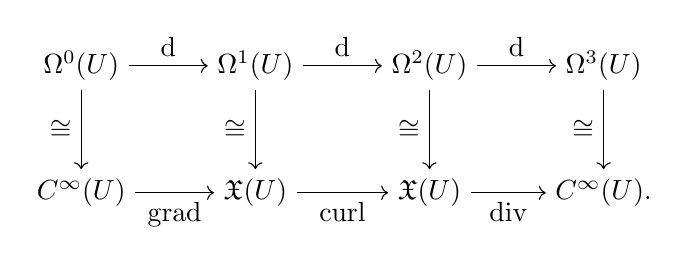
\begin{tikzpicture}
\node (omega0) {$\Omega^0(U)$};
\node (omega1) [right =of omega0] {$\Omega^1(U)$};
\node (omega2) [right =of omega1] {$\Omega^2(U)$};
\node (omega3) [right =of omega2] {$\Omega^3(U)$};
\node (cinfty) [below =of omega0] {$C^\infty(U)$};
\node (bigX) [below =of omega1] {$\XXX(U)$};
\node (bigx2) [below =of omega2] {$\XXX(U)$};
\node (cinfty2) [below =of omega3] {$C^\infty(U)$.};
\draw[->] (omega0) -- node[above] {d} (omega1);
\draw[->] (omega1) -- node[above] {d} (omega2);
\draw[->] (omega2) -- node[above] {d} (omega3);
\draw[->] (omega0) -- node[left] {$\cong$} (cinfty);
\draw[->] (omega1) -- node[left] {$\cong$} (bigX);
\draw[->] (omega2) -- node[left] {$\cong$} (bigx2);
\draw[->] (omega3) -- node[left] {$\cong$} (cinfty2);
\draw[->] (cinfty) -- node[below] {grad} (bigX);
\draw[->] (bigX) -- node[below] {curl} (bigx2);
\draw[->] (bigx2) -- node[below] {div} (cinfty2);
\end{tikzpicture}\\

\end{center}
Shorthand
\begin{align*}
	\sum_{i,j} a_ib_j &= \sum_i a_i\sum_j b_j\\
	\sum_{i,j} a_ib_j &= \sum_i a_i\sum_j b_j\\
	\sum_I a_I &= \sum_{n=1}^k a_{i_n}\\
	\sum_{I,J} a_I b_J &= \sum_{n=1}^k a_{i_n}\sum_{m=1}^k b_{j_m} \\
	\delta_i^j &= \BINDEF{1 & i=j}{0 & i \ne j}\\
	\delta_I^J &= \delta_{i_1}^{j_1}\delta_{i_2}^{j_2}\cdots\delta_{i_k}^{j_k} = \BINDEF{1 & i_n = j_n, \forall n}{0 & \text{otherwise}} = \BINDEF{1 & I=J}{0 & I \ne J}
\end{align*}

\begin{definition}[Exact and Closed $k$-forms]

A $k$-form $\omega$ on $U$ is \DEFINE{closed} if $d\omega=0$; it is \DEFINE{exact} if there is a $(k-1)$-form $\tau$ such that $\omega = d\tau$ on $U$.  Since $d(d\tau)=0$, every exact form is closed.  

\end{definition}

\begin{definition}[de Rham Cohomology].

The \DEFINE{$k\ITH$-cohomology of $U$} is defined as the quotient vector space
\begin{align*}
	H^k(U) = \frac{\{\text{closed k-forms}\}}{\{\text{exact k-forms}\}}
\end{align*}That is, each element is a vector space forming an equivalence class of $k$-forms.

\end{definition}

\textbf{Examples of de Rham Cohomology}\\

De Rham cohomology provides a way to study the topology of smooth manifolds using differential forms. Below are some key examples illustrating how to compute and interpret de Rham cohomology groups.

---
\begin{description}

\item \textbf{**Example 1: Euclidean Space \( \mathbb{R}^n \)** } \\
For \( M = \mathbb{R}^n \), we claim that the de Rham cohomology is:

\[
H^k_{\text{dR}}(\mathbb{R}^n) =
\begin{cases}
\mathbb{R}, & k = 0, \\
0, & k > 0.
\end{cases}
\]

**Computation**\\
\begin{enumerate}

\item **\( H^0_{\text{dR}}(\mathbb{R}^n) \):** 
\begin{itemize}
 
   \item  The 0-forms are just smooth functions \( f \).  \\
   \item A function is closed if \( df = 0 \), meaning \( f \) is constant.  \\
   \item Every constant function is not only closed but also exact since \( f = d(fx) \).  \\
   \item The space of closed 0-forms is \( \mathbb{R} \) (constant functions), and there are no exact forms to quotient out.  \\
   \item So, \( H^0_{\text{dR}}(\mathbb{R}^n) = \mathbb{R} \).\\

\end{itemize}
\item **\( H^k_{\text{dR}}(\mathbb{R}^n) \) for \( k > 0 \):**  \\
\begin{itemize}

   \item  Any closed \( k \)-form \( \omega \) is locally exact due to **Poincaré’s lemma**.  \\
   \item  That is, every closed form is of the form \( \omega = d\eta \), meaning it contributes nothing to cohomology.\\
   \item Thus, \( H^k_{\text{dR}}(\mathbb{R}^n) = 0 \) for \( k > 0 \).

This result reflects the fact that \( \mathbb{R}^n \) is **contractible**, so it has trivial topology.

\end{itemize}
\end{enumerate}

---\\

\item \textbf{ **Example 2: The Circle \( S^1 \)** }\\
 
For \( M = S^1 \), we find:

\[
H^k_{\text{dR}}(S^1) =
\begin{cases}
\mathbb{R}, & k = 0, 1, \\
0, & k > 1.
\end{cases}
\]

**Computation**\\
\begin{enumerate}

\item  **\( H^0_{\text{dR}}(S^1) = \mathbb{R} \)**  

\begin{itemize}

   \item  Smooth functions \( f \) that satisfy \( df = 0 \) are constant.
   \item  Thus, \( H^0_{\text{dR}}(S^1) = \mathbb{R} \).

\end{itemize}
\item  **\( H^1_{\text{dR}}(S^1) = \mathbb{R} \)**  \\
\begin{itemize}

   \item  Consider the 1-form \( \omega = d\theta \), where \( \theta \) is the angular coordinate.  
   \item  \( d\omega = 0 \), so \( \omega \) is closed.  \\
   \item  Is \( \omega \) exact? If \( \omega = d\eta \) for some \( \eta \), then \( d\eta = d\theta \), but no globally defined function \( \eta \) exists on \( S^1 \) satisfying this. \\ 
   \item  So \( \omega \) represents a **nontrivial cohomology class**, giving \( H^1_{\text{dR}}(S^1) = \mathbb{R} \).

\end{itemize}
\item  **\( H^k_{\text{dR}}(S^1) = 0 \) for \( k \geq 2 \)**  \\
   - There are no nontrivial 2-forms on a 1-dimensional manifold.

 **Interpretation**\\
 \begin{itemize}
\item  The nontrivial \( H^1_{\text{dR}}(S^1) \) reflects the existence of a **loop** in \( S^1 \).\\
\item  This cohomology detects the ability to define a **non-exact closed form**, related to the winding number.

\end{itemize}
\end{enumerate}
---

\item \textbf{ **Example 3: The 2-Sphere \( S^2 \)**  
For \( M = S^2 \):
}
\[
H^k_{\text{dR}}(S^2) =
\begin{cases}
\mathbb{R}, & k = 0, 2, \\
0, & k = 1.
\end{cases}
\]

 **Computation**\\
 
 \begin{enumerate}
 
\item  **\( H^0_{\text{dR}}(S^2) = \mathbb{R} \)**  \\
\begin{itemize}
   \item  As always, closed 0-forms are constant functions, so \( H^0_{\text{dR}}(S^2) = \mathbb{R} \)\\

\end{itemize}

\item  **\( H^1_{\text{dR}}(S^2) = 0 \)**  
\begin{itemize}
   \item  Any closed 1-form is exact by a higher-dimensional **Poincaré lemma**, so \( H^1_{\text{dR}}(S^2) = 0 \).\\

\end{itemize}

\item  **\( H^2_{\text{dR}}(S^2) = \mathbb{R} \)**  \\
\begin{itemize}
   \item  The standard volume form \( \omega = \sin\theta \, d\theta \wedge d\phi \) is closed.  \\
   \item  It is not exact, because there is no 1-form \( \eta \) such that \( d\eta = \omega \) (this follows from **Stokes’ theorem**).\\  
   \item  So \( \omega \) represents a generator of \( H^2_{\text{dR}}(S^2) \).

\end{itemize}
   
 \end{enumerate}

 **Interpretation**
\begin{itemize}
\item  \( H^1_{\text{dR}}(S^2) = 0 \) reflects that there are no **nontrivial loops** (all loops contract).
\item  \( H^2_{\text{dR}}(S^2) = \mathbb{R} \) corresponds to the existence of a volume form, a global topological feature.

\end{itemize}

---

\item \textbf{**Example 4: The Torus \( T^2 = S^1 \times S^1 \)**}  \\
For \( T^2 \), the de Rham cohomology groups are:

\[
H^k_{\text{dR}}(T^2) =
\begin{cases}
\mathbb{R}, & k = 0,2, \\
\mathbb{R} \oplus \mathbb{R}, & k = 1, \\
0, & k > 2.
\end{cases}
\]

 **Computation**\\
 
 \begin{enumerate}
 
\item  **\( H^0_{\text{dR}}(T^2) = \mathbb{R} \)** (constant functions).  \\
\item  **\( H^1_{\text{dR}}(T^2) = \mathbb{R} \oplus \mathbb{R} \)**  
\begin{itemize}
   \item  The torus has two independent 1-forms: \( d\theta_1 \) and \( d\theta_2 \), corresponding to the two loops in \( T^2 \).\\

\end{itemize}
\item  **\( H^2_{\text{dR}}(T^2) = \mathbb{R} \)**  
   \item The volume form \( d\theta_1 \wedge d\theta_2 \) represents a nontrivial 2-class.\\

 \end{enumerate}


 **Interpretation**\\
 \begin{itemize}
 
\item The rank of \( H^1_{\text{dR}}(T^2) \) reflects the **two independent loops** in the torus.\\
\item  The nontrivial \( H^2_{\text{dR}}(T^2) \) corresponds to the existence of a **volume form**.\\

 \end{itemize}

\end{description}
 ---

 **Summary Table**\\ \\
 \begin{tabular}{|c|c|c|c|}
 \hline
  Manifold M & $H^0_{dR}(M)$ & $H^2_{dR}(M)$& $H^1_{dR}(M)$ \\
 \hline
  \( \mathbb{R}^n \) & \( \mathbb{R} \) & 0 & 0 \\
 \hline
 \( S^1 \) & \( \mathbb{R} \) & \( \mathbb{R} \) & 0 \\
 \hline
  \( S^2 \) & \( \mathbb{R} \) & 0 & \( \mathbb{R} \) \\
 \hline
 \( T^2 \) & \( \mathbb{R} \) & \( \mathbb{R} \oplus \mathbb{R} \) & \( \mathbb{R} \)\\
 \hline
 \end{tabular}\\

\end{document}
